%\documentclass{article}
%\documentclass[hyperref={colorlinks=true}]{beamer}
\documentclass[handout,hyperref={colorlinks=true}]{beamer}

\usecolortheme{crane}
\usetheme{Darmstadt}
\usefonttheme{structuresmallcapsserif}
%%%%%%%%%%%%%%%%%%%%%%%%%%%%%%Paquetes%%%%%%%%%%%%%%%%%%%%%%%%%%%%%%%%%%%%%%%%%%%%%%%5
%%%%%%%%%%%%%%%%%%%%%%%%%%%%%%%%%%%%%%%%%%%%%%%%%%%%%%%%%%%%%%%%%%%%%%%%%%%%%%%%%%%%%
%\usepackage{pgfpages}
%\pgfpagesuselayout{2 on 1}[a4paper,border shrink=5mm]
\usepackage{empheq}
\usepackage[spanish]{babel}
\usepackage[utf8x]{inputenc}
\usepackage{times}
\usepackage[T1]{fontenc}
\usepackage{amssymb,amsmath}
\usepackage{enumerate}
\usepackage{verbatim}
\usepackage{ esint }
%\usepackage{pst-all}
%\usepackage{pstricks-add}
\usepackage{array}
%\usepackage[T1]{fontenc}
\usepackage{animate}
%\usepackage{media9}
\usepackage{xparse}
\usepackage{listings}
\usepackage{ wasysym }
\usepackage{sagetex}
\usepackage{yfonts,mathrsfs,eufrak}
\usepackage{hyperref}

%%%%%%%%%%%%%%%%%%%%%%%%%Configuracion listing
\lstdefinelanguage{Sage}[]{Python}
{morekeywords={False,sage,True},sensitive=true}
\lstset{
frame=none,
showtabs=False,
showspaces=False,
showstringspaces=False,
commentstyle={\ttfamily\color{dgreencolor}},
keywordstyle={\ttfamily\color{dbluecolor}\bfseries},
stringstyle={\ttfamily\color{dgraycolor}\bfseries},
language=Sage,
basicstyle={\fontsize{8pt}{8pt}\ttfamily},
aboveskip=.3em,
belowskip=0.1em,
numbers=none,
numberstyle=\footnotesize
}
%%%%%%%%%%%%%%%%%%%%%%%%Colores
\definecolor{myblue}{rgb}{.8, .8, 1}
\definecolor{dblackcolor}{rgb}{0.0,0.0,0.0}
\definecolor{dbluecolor}{rgb}{0.01,0.02,0.7}
\definecolor{dgreencolor}{rgb}{0.2,0.4,0.0}
\definecolor{dgraycolor}{rgb}{0.30,0.3,0.30}
\newcommand{\dblue}{\color{dbluecolor}\bf}
\newcommand{\dred}{\color{dredcolor}\bf}
\newcommand{\dblack}{\color{dblackcolor}\bf}
%%%%%%%%%%%%%%%%%%%%%%%%%%Nuevos comandos entornos%%%%%%%%%%%%%%%%%%%%%%%%%%%%%%%%
%%%%%%%%%%%%%%%%%%%%%%%%%%%%%%%%%%%%%%%%%%%%%%%%%%%%%%%%%%%%%%%%%%%%%%%%
\newenvironment{demo}{\noindent\emph{Dem.}}{$\square$ \newline\vspace{5pt}}
\newcommand{\com}{\mathbb{C}}
\newcommand{\dis}{\mathbb{D}}
\newcommand{\rr}{\mathbb{R}}
\newcommand{\oo}{\mathcal{O}}
\renewcommand{\emph}[1]{\textcolor[rgb]{1,0,0}{#1}}
\newcommand{\der}[2]{\frac{\partial #1}{\partial #2}}
\renewcommand{\v}[1]{\overrightarrow{#1}}
\renewcommand{\epsilon}{\varepsilon}
\newlength\mytemplen
\newsavebox\mytempbox
\makeatletter
\newcommand\mybluebox{%
\@ifnextchar[%]
{\@mybluebox}%
{\@mybluebox[0pt]}}
\def\@mybluebox[#1]{%
\@ifnextchar[%]
{\@@mybluebox[#1]}%
{\@@mybluebox[#1][0pt]}}
\def\@@mybluebox[#1][#2]#3{
\sbox\mytempbox{#3}%
\mytemplen\ht\mytempbox
\advance\mytemplen #1\relax
\ht\mytempbox\mytemplen
\mytemplen\dp\mytempbox
\advance\mytemplen #2\relax
\dp\mytempbox\mytemplen
\colorbox{myblue}{\hspace{1em}\usebox{\mytempbox}\hspace{1em}}}
\makeatother
\DeclareDocumentCommand\boxedeq{ m g }{%
{\begin{empheq}[box={\mybluebox[2pt][2pt]}]{equation}% #1%
\IfNoValueF {#2} {\label{#2}}%
#1
\end{empheq}
}%
}
\DeclareMathOperator{\atan2}{atan2}
\DeclareMathOperator{\sen}{sen}
\newtheorem{teorema}{Teorema}[section]
\newtheorem{lema}[teorema]{Lema}
\newtheorem{corolario}[teorema]{Corolario}
\newtheorem{proposicion}[teorema]{Proposici\'on}
\newtheorem{definicion}[teorema]{Definici\'on}
%%%%%%%%%%%%%%%%%%%%%%%%%%%%%%%%%%%%%%%%%%%%%%%%%%%%%%%%%%%%%%%%%%%%%%%%%%%%%%%%%%%%%%%%%%%%%%%%%%%%%%%%%%%
%%%%%%%%%%Para escibir en clase articulo o similar
% \usepackage{color}
% \newcommand{\nl}{ }
% \renewenvironment{frame}[1]{}{}
% \newcommand{\qed}{$\square$}
% %\newcommand{\defverbatim}{\def{#1}}
% \newenvironment{block}[1]{\textbf{#1}}{}
% \title{Ecuaciones lineales de segundo orden}
% \author{Fernando Mazzone}
%
%%%%%%%%%%%%%%%%%%%%%%%Para clase beamer
\newcommand{\nl}{\onslide<+-> }

\title[Teoría de Lie y ODE] % (optional, nur bei langen Titeln nötig)
{%
Cambios de variables, Teoría de Lie y EDO
}



\author[] % (optional, nur bei vielen Autoren)
{Fernando Mazzone}

\institute[Depto de Matemática] % (optional, aber oft nötig)
{
 Depto de Matemática\\
Facultad de Ciencias Exactas Físico-Químicas y Naturales\\
Universidad Nacional de Río Cuarto}


\subject{Ecuaciones Diferenciales}

%%%%%%%%%%%%%%%%%%%%%%%%%%%%%%%%%%%%%%%%%%%%%%%%%%%%%%%%%%%%%%%%%%%%%%%%%%%%%%%%%%%%%%


\begin{document}
\begin{frame}
  \maketitle
  \begin{center}
   
\includegraphics[scale=0.2]{imagenes/unrc.jpg}
   \end{center}
\end{frame}

\begin{frame}{Distintas formas para una ecuación}
Consideremos la ecuación diferencial general de primer orden 

\begin{equation}\label{eq:gral_orden1}
\frac{dy}{dx}=f(x,y)
\end{equation}
O su equivalente como forma diferencial
\begin{equation}\label{eq:gral_orden1_FormDif}
M(x,y)dx+N(x,y)dy=0
\end{equation}
 La expresión $\frac{dy}{dx}$ implica una asimetría entre las variables $x$ e $y$, una de ellas es independiente ($x$) y la otra ($y$) independiente.

La expresión  $M(x,y)dx+N(x,y)dy$ es más simétrica, las dos variables tienen el mismo estatus en la expresión.  Además las expresiones del tipo \eqref{eq:gral_orden1_FormDif} representan un ente matemático importante llamado \href{http://es.wikipedia.org/wiki/Forma_diferencial}{forma diferencial}


\end{frame}

\begin{frame}{Formas diferenciales, idea somera}


\begin{enumerate}
\item<+-> Como los polinomios, las formas diferenciales tienen grado. 
\item<+-> Dadas dos (pueden ser mas) variables $x,y$ una 0-forma diferencial es una función $g(x,y)$ de $x,y$. 
\item<+> La expresión \eqref{eq:gral_orden1_FormDif} es una 1-forma diferencial.
\item<+-> Hay un operador llamado diferencial y denotado por $d$. Si $\omega$ es una $k$-forma diferencial $d\omega$ es una $k+1$ forma diferencial.
\item<+-> En el caso de $0$-forma (función) $g(x,y)$ el diferencial se define
\[dg=\frac{\partial M}{\partial x}dx+ \frac{\partial N}{\partial y}dy.\]
Una $k$-forma diferencial se llama exacta cuando es el diferencial de una $k-1$-forma.
\end{enumerate}


\end{frame}

\begin{frame}{Cambios de variables}

\begin{block}{Idea básica}
 Suṕongamos la ecuación \eqref{eq:gral_orden1} o \eqref{eq:gral_orden1_FormDif} en las variables $x,y$. La idea es encontrar nuevas variables $\xi=\xi(x,y)$ y $\eta=\eta(x,y)$ tales que la ecuación se transforme en una más sencilla de resolver. 
\end{block}




\end{frame}

\begin{frame}{Cómputos de cambiamos variables}
\textbf{Cambio de la variable dependiente $y=h(x,z)$ manteniendo la independiente} 

\[\frac{dy}{dx}=\frac{\partial h}{\partial x}+\frac{\partial h}{\partial z}\frac{dz}{dx}.\]

La ecuación se convierte

\[\frac{\partial h}{\partial x}+\frac{\partial h}{\partial z}\frac{dz}{dx}=f(x,h(x,z)).\]

Que es una expresión sólo en $z$ y $x$. Parece más complicada, pero en un ejemplo concreto puede ser más simple.



\end{frame}

\begin{frame}{Cómputos de cambios de variables, ejemplo}

\textbf{Ejemplo 1} Hacer el cambio de variable en la  ecuación 

\[y=\frac{e^z}{x}\quad\text{en}\quad  y'=\left[\ln(xy)\right]^2xy-\frac{y}{x}.\]
1) Expresemos $dy/dx$ sólo con $x$ y $z$ y $dz/dx$.
\[\frac{dy}{dx}=-\frac{e^z}{x^2}+\frac{e^z}{x}\frac{dz}{dx}.\]
2) Remplacemos $y'$ e $y$ en la ecuación 
\[-\frac{e^z}{x^2}+\frac{e^z}{x}\frac{dz}{dx}=\left[\ln\left(x \frac{e^z}{x} \right)\right]^2x\frac{e^z}{x}-\frac{\frac{e^z}{x} }{x}.\]
3) Simplifiquemos
\[\frac{dz}{dx}=z^2x.\]
Que es una ecuación muy facil de resolver.


\end{frame}










\begin{frame}[fragile]{Cómputos de cambios de variables, ejemplo}
Lo podemos hacer con \texttt{SymPy}

\begin{sageblock}
from sympy import *
x,y,z=symbols('x,y,z')
y=Function('y')(x)
z=Function('z')(x)
y=exp(z)/x
eq=Eq(y.diff(x)-(ln(x*y))**2*x*y+y/x,0)
simplify(eq)
\end{sageblock}
Obtenemos la ecuación
\[\sage{simplify(eq)}\]
que \texttt{SymPy} no simplifica a nuestro gusto
\end{frame}



\begin{frame}{Cómputos de cambios de variables}
\textbf{Cambio de la variable independiente $t=h(x)$ manteniendo la dependiente} 

\[\frac{dy}{dx}=\frac{dy}{dt}\frac{dh}{dx}=\frac{dy}{dt}h'(x).\]

Suponiendo $h$ biyectiva, la ecuación se convierte

\[\frac{dy}{dt}h'(h^{-1}(t))=f(h^{-1}(t),y).\]

Que es una expresión sólo en $t$ e $y$. 



\end{frame}

\begin{frame}{Cómputos de cambios de variables, ejemplo}

\textbf{Ejemplo 2} Hacer el cambio de variable en la  ecuación 
\[x=\cos t\quad\text{en}\quad  -\frac{dy}{dx}+\frac{1}{\sqrt{1-x^2}}y=0.\]
1) $h(x)=\arcsen x$
\[\frac{dy}{dx}=\frac{dy}{dt}h'(x)=-\frac{1}{\sqrt{1-x^2}}\frac{dy}{dt}.\]
2) Remplacemos $x$ e $y'$ en la ecuación 
\[\frac{1}{\sqrt{1-x^2}}\frac{dy}{dt}+ \frac{1}{\sqrt{1-x^2}}y=0\]
3) Simplificando
\[\frac{dy}{dt}+ y=0\]
Que es una ecuación lineal a coeficientes constantes.


\end{frame}

\begin{frame}[fragile]{Cómputos de cambios de variables, ejemplo}
Lo podemos hacer con \texttt{SymPy}

\begin{sageblock}
from sympy import *
x,t=symbols('x,t')
t=acos(x)
y=Function('y')(t)
Ecuacion=-y.diff()+1/(sqrt(1-x**2))*y
\end{sageblock}
Obtenemos la ecuación
\[\sage{simplify(Ecuacion)}=0\]
Nuevamente \texttt{SymPy} no simplifica a nuestro gusto
\end{frame}

\begin{frame}{Cambios de variables}
\textbf{Cambio de variable general $\xi=\xi(x,y)$, $\eta=\eta(x,y)$}

1) Calculamos $d\eta/d\xi$ en las variables $x,y$
\begin{equation}\label{eq:subsder}
\frac{d\eta}{d\xi}=\frac{\frac{d\eta}{dx}}{\frac{d\xi}{dx}}=\frac{\frac{\partial\eta}{\partial x}+\frac{\partial\eta}{\partial y}y'}{\frac{\partial\xi}{\partial x}+\frac{\partial\xi}{\partial y}y'}=\frac{\frac{d\eta}{dx}}{\frac{d\xi}{dx}}=\frac{\frac{\partial\eta}{\partial x}+\frac{\partial\eta}{\partial y}f(x,y)}{\frac{\partial\xi}{\partial x}+\frac{\partial\xi}{\partial y}f(x,y)}.
\end{equation}

2) En la expresión resultante sustituir $x,y$ por las tansformaciones inversas $x=x(\xi,\eta)$ y  $y=y(\xi,\eta)$


\end{frame}


\begin{frame}[fragile]{Cambios de variables}
\textbf{Ejemplo 3. Transformar a polares:} $\frac{dy}{dx}=\frac{y^3+x^2y-x-y}{x^3+xy^2-x+y}.$

Dado que el cálculo es extenso lo haremos sólo con \texttt{SymPy}
\begin{sageblock}
from sympy import *
x=symbols('x')
y=Function('y')(x)
r=sqrt(x**2+y**2)
theta=atan(y/x)
Expr2=r.diff(x)/theta.diff(x)
Expr3=Expr2.subs(y.diff(x),\
(y**3+x**2*y-x-y)/(x**3+x*y**2-x+y))
r,theta=symbols('r,theta',positive=True)
Expr4=Expr3.subs([(y,r*sin(theta)),\
(x,r*cos(theta))])
Expr5=simplify(Expr4)
\end{sageblock}
\end{frame}

\begin{frame}[fragile]{Cambios de variables}
Encontramos que en polares la ecuación es mucho más simple
\[\frac{dr}{d\theta}=\sage{powsimp(Expr5)}.\]

\end{frame}



\begin{sagesilent}
reset()
\end{sagesilent}


\begin{frame}[fragile]{Cambios de variables con \texttt{SAGE} y formas diferenciales}
\texttt{SAGE} puede operar con formas diferenciales
\begin{sagecommandline}
sage: r,theta=var('r,theta')
sage: U = CoordinatePatch((r,theta))
sage: F = DifferentialForms(U)
sage: x= DifferentialForm(F, 0, r*cos(theta))
sage: y= DifferentialForm(F, 0, r*sin(theta))
sage: w=(x^3+x*y^2-x+y)*y.diff()-(y^3+x^2*y-x-y)*x.diff()
sage: w[0].simplify_full()
sage: w[1].simplify_full()
\end{sagecommandline}
La forma obtenida es $\sage{w[0].simplify_full()}dr+(\sage{w[1].simplify_full()})d\theta$.
\end{frame}




\begin{frame}{Grupos, Repaso}
\begin{block}{Grupos}
Sean $G$ un conjunto y $\alpha$ una función tal que   $\alpha:G\times G\to G$. En el contexto de grupos es más usual la notación  $\alpha(g_1,g_2)=g_1g_2$. El par $(G,\alpha)$ se llama un grupo si se satisface
\begin{enumerate}
\item $(g_1g_2)g_3=g_1(g_2g_3)$, para todos $g_1,g_2,g_3\in G$,
\item Existe $e\in G$ tal que $eg=ge=g$,  para todo $g\in G$.
\item Para todo $g\in G$ existe $h\in G$ tal que $gh=hg=e$. Se acostumbra denotar $h=g^{-1}$.
\end{enumerate}
\end{block}


\end{frame}



\begin{frame}{Ejemplos de grupos}
\nl\textbf{Ejemplo 1} Sea $\Pi$ un plano euclideano y $G$ el conjunto de todas las transformaciones rígidas de $\Pi$ en si mismo. Entonces $G$ es un grupo con la operación de composición. Se llama el \emph{grupo de transformaciones rígidas}

\nl\textbf{Ejemplo 2} Sea $X=\{x_1,\ldots,x_n\}$ un conjunto de $n$ elementos y $S_n$ definido por 
\[S_n=\{\sigma|\sigma:X\to X\hbox{ y }\sigma \hbox{ es biyectiva }\}\]
Entonces $S_n$ es un grupo  con la operación de composición. Se denomina \href{http://es.wikipedia.org/wiki/Grupo_simétrico}{\emph{grupo simétrico}} 
\end{frame}

\begin{frame}{Ejemplos de grupos}
\nl\textbf{Ejemplo 3} Sea $\Delta$ un polígono regular de $n$ lados  en un plano euclideano $\Pi$ y $D_{2n}$ el conjunto de todas las transformaciones rígidas de $\Pi$ en si mismo que llevan $\Delta$ en si mismo. $D_{2n}$ se llama el \href{http://es.wikipedia.org/wiki/Grupo_diedral}{\emph{grupo diedral}}  de orden $2n$.
Para un triángulo equilatero
\href{http://es.wikipedia.org/wiki/Grupo_diedral}{\emph{grupo diedral}}

\begin{center}
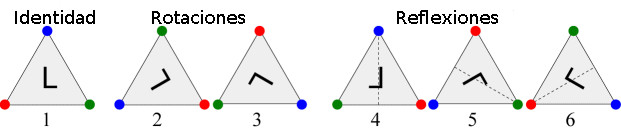
\includegraphics[scale=.4]{imagenes/SimTria.jpg}
\end{center}

\end{frame}



\begin{frame}{Teoría de grupos computacional: SAGE y GAP}

\href{http://www.gap-system.org/}{GAP - Groups, Algorithms, Programming} Lenguaje de programación para algebra discreta

\href{http://www.sagemath.org/}{SAGE:}  es un sistema de software de matemáticas libre de código abierto bajo la licencia GPL. Se basa en  muchos paquetes de código abierto existentes: NumPy, SciPy, matplotlib, SymPy, Maxima, GAP, FLINT, R y muchos más. Acceda a su poder combinado a través de un lenguaje común, basado en Python 
Misión: Creación de una alternativa libre de código abierto viable a Magma, Maple, Mathematica y Matlab.


\end{frame}

\begin{sagesilent}
reset()
\end{sagesilent}

\begin{frame}[fragile]{Teoría de grupos computacional: SAGE y GAP}
\begin{sagecommandline}
sage: G=SymmetricGroup(5)
sage: sigma=G([(1,2,3),(4,5)])
sage: sigma^2
sage: sigma^3
sage: sigma^6
sage: G.order()
sage: H=G.subgroup([sigma])
sage: H.order()
\end{sagecommandline}
\end{frame}


\begin{frame}[fragile]{Teoría de grupos computacional: SAGE y GAP}
\begin{sagecommandline}
sage: H.list()
sage: H.is_normal()
sage: G1=DihedralGroup(3)
sage: G1[-2]
sage: H1=G1.subgroup(G1[-2])
sage: H1.is_normal()
sage: G1.quotient(H1)
\end{sagecommandline}
\end{frame}

\begin{frame}{Grupos de simetrías}
\nl\begin{block}{Grupos de simetrías}
Los cambios de variables de un conjunto de dos variables, digamos $x$ e $y$, son funciones $\varphi$, invertibles,  de clase $C^{\infty}$, donde $\varphi:\Omega_1\to\Omega_2$, con $\Omega_1,\Omega_2$ abiertos de $\rr^2$. Acostumbraremos escribir $(\xi,\eta)=\varphi(x,y)$ y diremos que $(\xi,\eta)$ son la variables nuevas e $(x,y)$ las viejas.

Llamaremos $\mathscr{T}$ al conjunto de todas los cambios de variables $\varphi$. 
El conjunto  $\mathscr{T}$ tiene una estructura de grupo con la operación de composición.


\end{block}


\end{frame}


\begin{frame}{Grupos de simetrías, ejemplos}
\textbf{Ejemplo, polares:} Es más facil describir la transformación que lleva coordenadas polares en cartesinas. En este caso $(x,y)=\varphi(r,\theta)$ y
\[
\begin{array}{ll}
\varphi(r,\theta)&=(r\cos(\theta),r\sen(\theta)),\\
\Omega_1&=(0,\infty)\times (-\pi,\pi),\\
\Omega_2&=\rr^2-\{(x,y)|y=0,x\leq 0\}\\
\end{array}
\]

\end{frame}

\begin{frame}{Grupos de Lie uniparamétricos}
\nl\begin{block}{Grupos uniparamétricos de simetrías}
Sea $\mathscr{T}$ el grupo de cambios de variables. Supongamos dado un homomorfismo de grupos $P:(\rr,+)\to (\mathscr{T},\circ)$.  

\textbf{Notación:} 
\begin{enumerate}
\item Para $\lambda\in\rr$ escribiremos $P_{\lambda}=P(\lambda)$ 
\item Si $(x,y)\in\rr^2$ escribimos $(\xi,\eta)=f(x,y,\lambda):=P_{\lambda}(x,y)$.
\end{enumerate}
Si $f(x,y,\lambda)$ es diferenciable respecto a $(x,y)$ y analítica respecto a $\lambda$ diremos que $\{P_{\lambda}|\lambda\in\rr\}$ es un \href{http://es.wikipedia.org/wiki/Grupo_uniparamétrico}{\emph{grupo de Lie uniparamétrico de simetrías}}.
\end{block}


\end{frame}






\begin{frame}{Grupos de Lie uniparamétricos}
\nl\begin{block}{Propiedades de $P_{\lambda}$}
\begin{enumerate}
\item<+->$P_{\lambda}$ es biyectiva y diferenciable sobre su domio de definición en su imagen.
 \item<+-> $P_{\lambda_1}\circ P_{\lambda_2}=P_{\lambda_1+\lambda_2}$, equivalentemente $f(f(x,y,\lambda_1),\lambda_2)=f(x,y,\lambda_1+\lambda_2)$.

\item<+-> $P_0=I$, o $f(x,y,0)=(x,y)$.

\item<+-> $\left(P_{\lambda}\right)^{-1}=P_{-\lambda}$

\item<+-> Si $P_{\lambda}(x,y)=(\xi,\eta)$, entonces  $\xi(x,y,\lambda)$ y $\eta(x,y,\lambda)$ son  diferenciables respecto $(x,y)$ y se desarrollan en serie de potencias respecto a $\lambda$. Es decir para todo $\lambda_0\in\rr$ 
\[
\begin{array}{cc}
\xi(x,y,\lambda)&=a_0(x,y)+a_1(x,y)(\lambda- \lambda_0)+\cdots\\
\eta(x,y,\lambda)&=b_0(x,y)+b_1(x,y)(\lambda- \lambda_0)+\cdots\\
\end{array}
\]

\end{enumerate}

\end{block}


\end{frame}


\begin{frame}{Ejemplos grupos de Lie uniparamétricos}
\textbf{Ejercicio:} Demostrar que las siguientes aplicaciones inducen grupos de Lie uniparamétricos
\begin{enumerate}
\item<+-> $P_{\lambda}(x,y)=(x+\lambda,y)$ y $P_{\lambda}(x,y)=(x,y+\lambda)$.
\item<+-> $P_{\lambda}(x,y)=(e^{\lambda}x,y)$
\item<+->$P_{\lambda}(x,y)=\left(\frac{x}{1-\lambda x},\frac{y}{1-\lambda x} \right)$
\item<+->$P_{\lambda}(x,y)=\begin{pmatrix} \cos(\lambda) & -\sen(\lambda)
\\ \sen(\lambda) & \cos(\lambda)
\end{pmatrix} \begin{pmatrix} x\\ y
\end{pmatrix}
$
\end{enumerate}

\end{frame}



\begin{frame}{Grupo de simetrías de una ecuación}

\begin{block}{Definición}
Consideremos una ecuación
\[y'=f(x,y).\]
Una transformación $P\in \mathscr{T}$ se denomina una simetría de la ecuación si el cambio de variables dado por $(\xi,\eta)=P(x,y)$ deja invariante  la ecuación. 

\textbf{Ejercicio:} el conjunto de todas las simetría de una ecuación es un subgrupo de  $( \mathscr{T},\circ)$. Lo llamaremos \emph{grupo de simetrías} de la ecuación.

 

\end{block}


\end{frame}

 \begin{frame}{Encontrar simetrías}
 \textbf{Ejemplo: hallar simetrías de }
\[\frac{dy}{dx}=f(x).\]

De acuerdo con \eqref{eq:subsder} se debe cumplir que 
 \[\frac{\frac{\partial\eta}{\partial x}+\frac{\partial\eta}{\partial y}f(x)}{\frac{\partial\xi}{\partial x}+\frac{\partial\xi}{\partial y}f(x)}=f(\xi)\]

 Parece que debemos hacer las elecciones
   \[\boxed{\xi=x},\quad \frac{\partial\eta}{\partial x}=\frac{\partial\xi}{\partial y}=0,\quad
   \frac{\partial\eta}{\partial y}=\frac{\partial\xi}{\partial x}. \]
 Luego 
\[\frac{\partial\eta}{\partial y}=1\Rightarrow \boxed{\eta=y+\lambda} \]
con $\lambda$ constante arbitraria.
 \end{frame}

\begin{frame}{Encontrar simetrías}
Hallamos que el 
\[P_{\lambda}(x,y)=(x,y+\lambda)\]
es un grupo uniparamétrico de simetrías. De manera similar
\[P_{\lambda}(x,y)=(x+\lambda,y)\]
es un grupo uniparamétrico de simetrías para 
\[\frac{dy}{dx}=f(y).\]
Geométricamente en el primer caso todas las soluciones seobtienen trasladando una cualquiera verticalmente y en el segundo caso horizontalmente.

\end{frame}

\begin{frame}{Encontrar simetrías}

\begin{tabular}{cc}
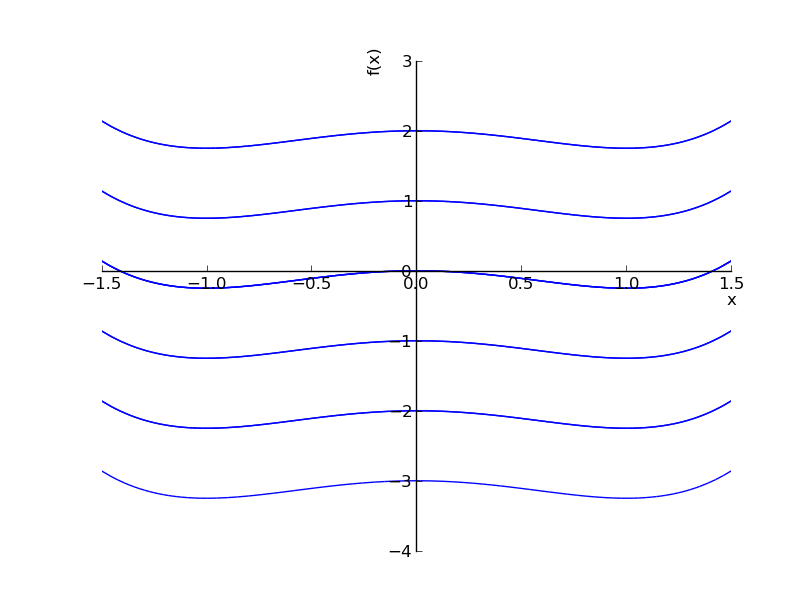
\includegraphics[scale=.3]{imagenes/sol_paralelas.png} &\hspace{-1.5cm}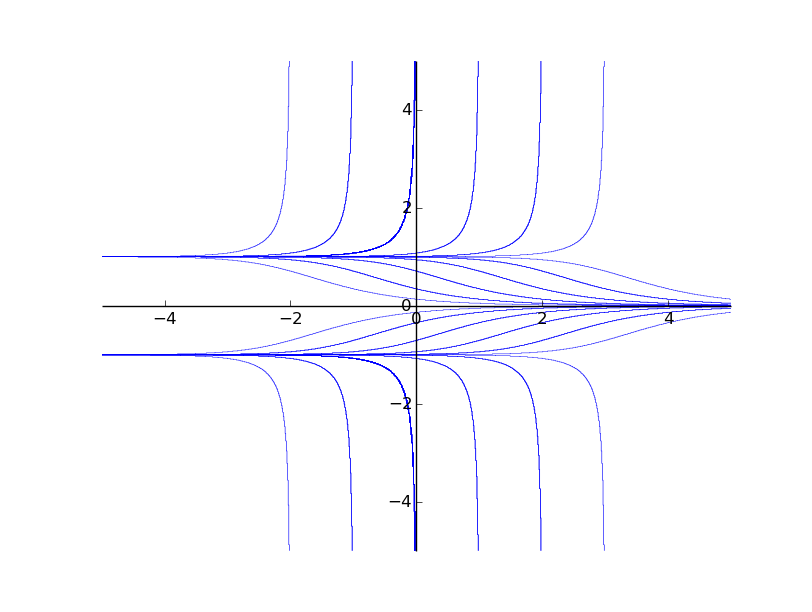
\includegraphics[scale=.3]{imagenes/sol_paralelas2.png} \\
Soluciones de $y'=x^3-x$ &\hspace{-1.5cm}Soluciones de $y'=y^3-y$
\end{tabular}

\end{frame}



\begin{frame}{Encontrar simetrías}
\textbf{Demostrar que las rotaciones alrededor del origen es un grupo uniparamétrico de simetrías de}
 \[\frac{dy}{dx}=\frac{y^3+x^2y-x-y}{x^3+xy^2-x+y}.\]
Sea $P_{\lambda}$ la transformación que rota un ángulo $\lambda$ alrededor del origen. Era un ejercicio demostrar que  $\{P_{\lambda}|\lambda\in\rr\}$ es un grupo uniparamétrico de simetrías. Se tiene la representación matricial
\[
P_{\lambda}(x,y)= \begin{pmatrix} \xi\\ \eta
\end{pmatrix}=\begin{pmatrix} \cos(\lambda) & -\sen(\lambda)
\\ \sen(\lambda) & \cos(\lambda)
\end{pmatrix} \begin{pmatrix} x\\ y
\end{pmatrix}
\]

\[
P^{-1}_{\lambda}(\xi,\eta)= \begin{pmatrix} x\\ y
\end{pmatrix}=\begin{pmatrix} \cos(\lambda) & \sen(\lambda)
\\ -sen(\lambda) & \cos(\lambda)
\end{pmatrix} \begin{pmatrix} \xi\\ \eta
\end{pmatrix}
\]



\end{frame}


\begin{frame}[fragile]{Encontrar simetrías}
 Para el cálculo recurrimos a \texttt{SymPy}
\begin{sageblock}
from sympy import *
x,theta=symbols('x,theta')
y=Function('y')(x)
xi=cos(theta)*x-sin(theta)*y
eta=sin(theta)*x+cos(theta)*y
Expr2=eta.diff(x)/xi.diff(x)
Expr3=Expr2.subs(y.diff(),\
(y**3+x**2*y-x-y)/(x**3+x*y**2-x+y))
xi,eta=symbols('xi,eta')
Expr4=Expr3.subs([(y, -sin(theta)*xi+cos(theta)*eta),\
(x,cos(theta)*xi+sin(theta)*eta)])
Expr5=simplify(Expr4)
Expr6=simplify(Expr5)
Expr7=Expr6.subs([(sin(2*theta + pi/4),sin(2*theta)*sqrt(2)+cos(2*theta)*sqrt(2))  , (cos(2*theta),1+(cos(theta))**2),(sin(2*theta),1-(cos(theta))**2)])
\end{sageblock}
\end{frame}

\begin{frame}[fragile]{Encontrar simetrías}
Tiene problemas para simplificar, lo tenemos que ayudar
\begin{sageblock}
Expr5=simplify(Expr4)
Expr6=Expr5.subs(sin(2*theta + pi/4),\
sin(2*theta)*sqrt(2)+cos(2*theta)*sqrt(2))
Expr7=Expr6.subs(cos(2*theta),\
1+(cos(theta))**2   )
Expr8=Expr7.subs(cos(2*theta),\
1+(cos(theta))**2)
Expr9=Expr8.subs(sin(2*theta),\
1-(cos(theta))**2)
\end{sageblock}
La ecuación resultante es \emph{la misma}
\boxedeq{\frac{d\eta}{d\xi}=\sage{simplify(Expr9)}.}{}
\end{frame}

\begin{frame}{Encontrar simetrías}
A la misma cocnclusión arribábamos si observamos que en en coordenadas polares la ecuación se escribe
\[\frac{dr}{d\theta}=r-r^3,\]
y que esta ecuación tiene las simetrías $P_{\lambda}:(r,\theta)\mapsto (r,\theta+\lambda)$. 
% \end{frame}


% \begin{frame}{Encontrar simetrías}


\vspace{1cm}
\begin{tabular}{p{6cm} p{4cm}}
\vspace{-3cm}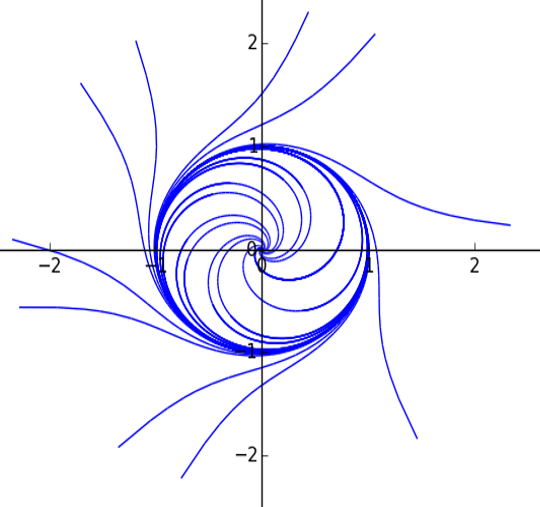
\includegraphics[scale=.4]{imagenes/sol_rotadas.png}&
\begin{minipage}[b]{4cm} Si rotamos un ángulo fijo el gráfico de una solución obtenemos el gráfico de otra solución.
\end{minipage}
  \\
\end{tabular} 
\end{frame}













% \begin{frame}{Acción de grupos}
% \begin{block}{Acción de grupos}
% Sea $G$ un grupo   y $X$ un conjunto. Diremos que $G$ actúa a izquierda sobre $X$ si existe una función $\alpha:G\times X\to X$, denotada $\alpha(g,x)=gx$ con las propiedades
% \begin{enumerate}
% \item $ex=x$,  donde $e$ neutro de $G$ y $x\in X$.
% \item $g(hx)=(gh)x$, donde $g,h\in G$ y $x\in X$ .
% \end{enumerate}
% \end{block}

% \nl\begin{block}{Acción de grupos}
% Si $G$ actúa a izquierda sobre $X$ y $x\in X$ definimos la \emph{órbita} de $x$ como el conjunto $\{gx|g\in G\}$. Denotamos la órbita de $x$ por $Gx$.
% \end{block}
% \end{frame}


% \begin{frame}[fragile]{Cambios de variables con \texttt{SAGE} y formas diferenciales}
% \begin{sagecommandline}
% sage: var('r,theta')
% sage: U = CoordinatePatch((r,theta))
% sage: F = DifferentialForms(U)
% sage: x= DifferentialForm(F, 0, r*cos(theta))
% sage: y= DifferentialForm(F, 0, r*sin(theta))
% sage: w=(x^3+x*y^2-x+y)*y.diff()-(y^3+x^2*y-x-y)*x.diff()
% sage: w[0].simplify_full()
% sage: w[1].simplify_full()
% \end{sagecommandline}
% La forma obtenida es $\sage{w[0].simplify_full()}dr+(\sage{w[1].simplify_full()})d\theta$.
% \end{frame}


\end{document}
